\documentclass{beamer}

\usepackage[utf8]{inputenc}
\usetheme{Warsaw}

\title{Embedded Systems - Bachelor Project}
\author{Moritz Herzog, Philipp Lersch}
\date{\today}

\usepackage{tikz}
\usetikzlibrary{shapes.geometric, arrows, chains, calc}


\addtobeamertemplate{navigation symbols}{}{%
    \usebeamerfont{footline}%
    \usebeamercolor[fg]{footline}%
    \hspace{1em}%
    \insertframenumber/\inserttotalframenumber
}

\AtBeginSection[]
{
  \begin{frame}
    \frametitle{Table of Contents}
    \tableofcontents[currentsection]
  \end{frame}
}
\renewcommand{\thefootnote}{\fnsymbol{footnote}}
\begin{document}
\maketitle


\section{OpenCL}
\begin{frame}
    \frametitle{OpenCL Structure}
    \begin{columns}
        \column{.6\textwidth}
        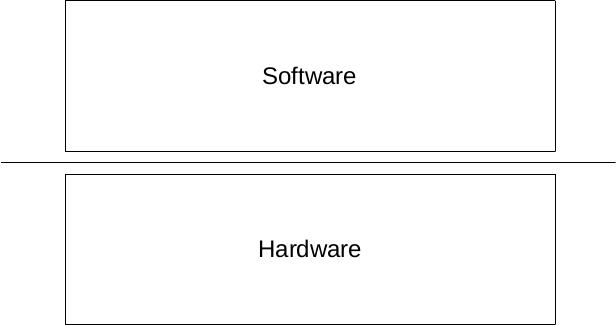
\includegraphics[width=\textwidth]{res/HardwareSoftwareLayer.jpg}
        \column{.4\textwidth}
        \begin{itemize}
            \item OpenCL draws clear line between hardware and software
            \begin{itemize}
		\item broad range of architectures
		\item scalebility
		\item compatility
		\item less code changes
	 \end{itemize}
        \end{itemize}
    \end{columns}
\end{frame}
\subsection{Hardware Model}
\begin{frame}
    \frametitle{Hardware Model - General}
    OpenCL Propertys:
    \begin{itemize}
     	\item One CPU-Based Host controlls multible Compute Devices
     	\item A Compute Device is every OpenCL complient connected GPU, CPU and FPGA and even more.
     	\item A Compute Device has one or more Compute Unit(s)
     	\item Processing Elements all execute OpenCL Kernels
	\item Diffrent models for CPU and GPU.
    \end{itemize}
\end{frame}
\begin{frame}
    \frametitle{Hardware Model - General}
    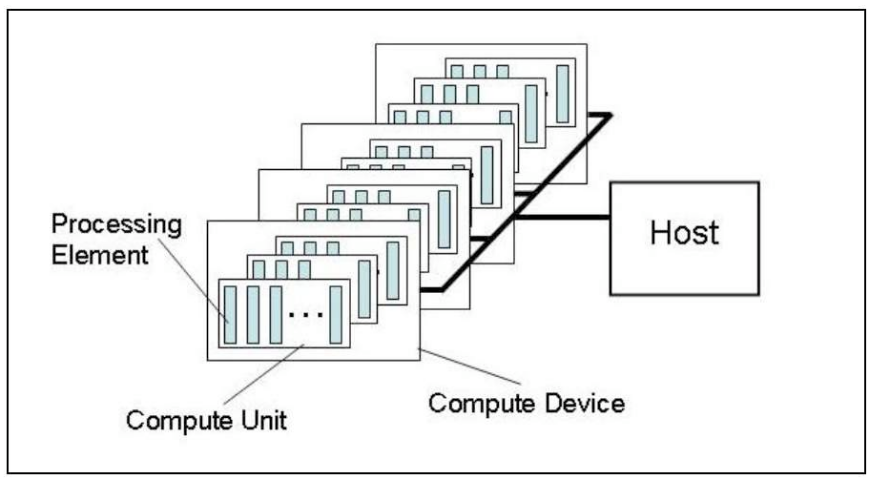
\includegraphics[width=\textwidth]{res/KhronosPlatformModel.png}
\end{frame}

\begin{frame}
    \frametitle{Hardware Model - Memory}
        \begin{itemize}
            \item Private Memory
            \begin{itemize}
             \item Private for every Workitem
            \end{itemize}
            \item Local Memory
            \begin{itemize}
             \item Shared within the Workgroup
            \end{itemize}
            \item Global/Constant Memory
            \begin{itemize}
             \item Visible for all Workgoups within the device
            \end{itemize}
            \item Host Memory
            \begin{itemize}
             \item Local DRAM
            \end{itemize}
            \item Memorymanagement can be explicit.
        \end{itemize}
\end{frame}
\begin{frame}
    \frametitle{Hardware Model - Memory}
        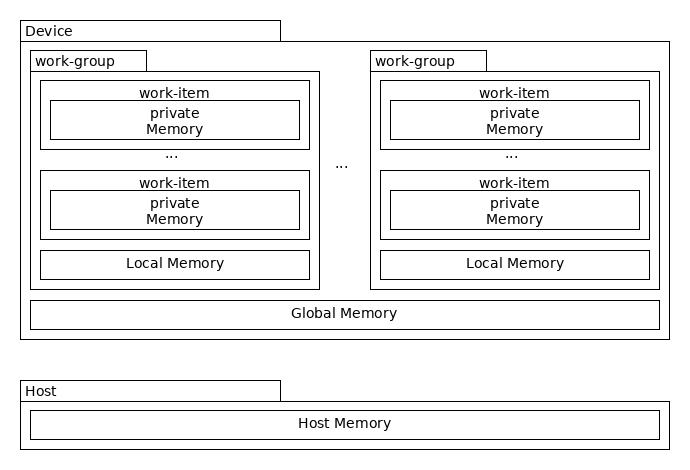
\includegraphics[width=.8\textwidth]{res/OpenCLMemoryStructure.jpg}
        
\end{frame}
\begin{frame}
    \frametitle{Hardware Model - CPU}
    Architecure:
    \begin{itemize}
        \item Processing Units are the Treads/Cores
        \item Out-of-order execution is possible
        \item Contains branch prediction
    \end{itemize}
    Benefits
    \begin{itemize}
        \item Benefits from idependant instruction in a kernel.
    \end{itemize}
\end{frame}

\begin{frame}
    \frametitle{Hardware Model - GPU}
    Architecure:
    \begin{itemize}
     \item Processing Unit are the streaming multiprocessors
     \item Specific Definition of Processing Units depends on the Hardware Vendor and generation
     \item A Processing Unit has mutlible cores
    \end{itemize}
    Benefits:
    \begin{itemize}
     \item GPU-Architecure benefits from small, sequential and highly parallel Workloads.
    \end{itemize}
\end{frame}

\begin{frame}{Example Raspberry Pi 3B+}
    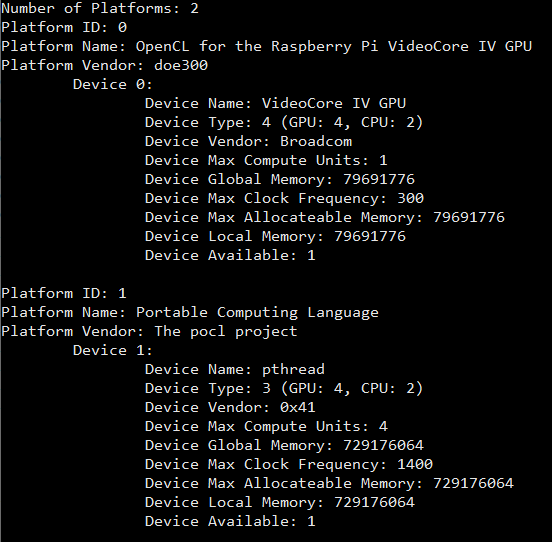
\includegraphics[height=.8\textheight]{res/RaspberryPiData.PNG}
\end{frame}
\subsection{Software Model}
\begin{frame}
    \frametitle{Software Model: Kernel}
        Kernel
        \begin{columns}
        \column{.6\textwidth}
            \begin{itemize}
            \item Aims for SIMD/SIMT\\
            $\Rightarrow$ Data/Thread Parallism
            \item describes thread behavior\\
            $\Rightarrow$ filled with data a single thread is called work item
            \item written in simplified C99 code\\
            $\Rightarrow$ kept simple for architectual flexibility
            \end{itemize} 
        \column{.4\textwidth}
            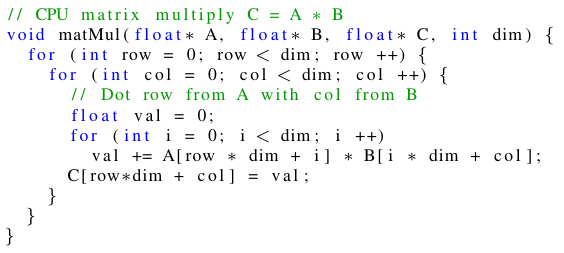
\includegraphics[width=\textwidth]{res/CodeExample.png}   
    \end{columns}
\end{frame}
\begin{frame}
    \frametitle{Software Model: Workgroup}
        Workgroup
        \begin{columns}
        \column{.6\textwidth}
            \begin{itemize}
            \item A set of multi dimensional arrays of work items\\
            \item in group syncable / outside independent
            \item exploids intstruction uniformity and memory contexts
            \end{itemize} 
        \column{.4\textwidth}
            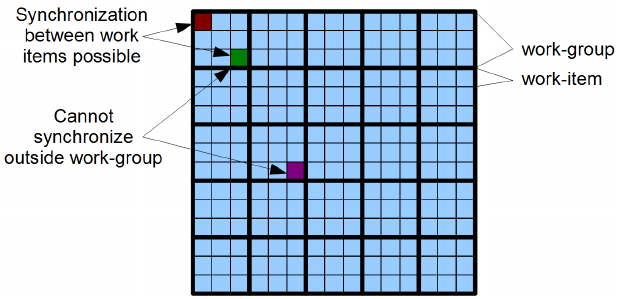
\includegraphics[width=\textwidth]{res/WorkGroupItemStructure.png}   
    \end{columns}
\end{frame}
\begin{frame}
    \frametitle{Software Model: Workgroup}
    \begin{columns}
        \column{.4\textwidth}
            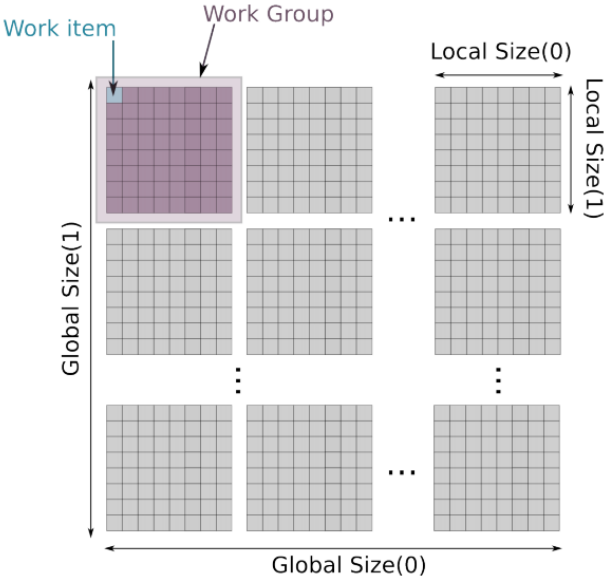
\includegraphics[width=\textwidth]{res/2DDataParallelWorkgroup.png}  
        \column{.6\textwidth}
            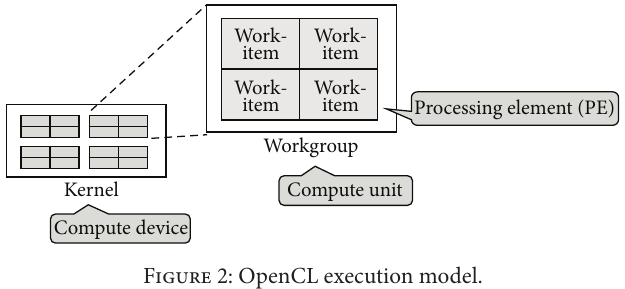
\includegraphics[width=\textwidth]{res/ExecutionModel.png}   
    \end{columns}
\end{frame}
\begin{frame}
    \frametitle{Software Model: Scheduler}
    Reminder: OpenCL builds on SIMT/D\\
    To map kernels efficently to hardware:\\
    $\Rightarrow$ workgroup size is important
    \begin{itemize}
        \item GPU: Many short Kernels/Threads\\
             $\Rightarrow$ Thread / Data Level Parallism
        \item CPU: Fewer longer, more complex Kernels/Threads\\
             $\Rightarrow$ Instruction Level Parallism\\
             $\Rightarrow$ CPU drowns in overhead in default implementations\\
             $\Rightarrow$ possible Solution: Kernel Serialization
    \end{itemize}
\end{frame}

\section{Kernels}
\subsection{Overview}
\begin{frame} %%Eine Folie
  \frametitle{List of Kernels} %%Folientitel
  Already there:
  \begin{itemize}
   \item Battery
   \item Speed
   \item Acceleration
   \begin{itemize}
    \item X-Achsis
    \item Y-Achsis
    \item Tangential
   \end{itemize}
   \item Tempreture
  \end{itemize}
\end{frame}
\begin{frame}
    \frametitle{List of Kernels}
    Added Kernels:
    \begin{itemize}
     \item Abnormal Acceleration Detection
     \item Tractioncontrol
     \item Range
     \item Turningradius
    \end{itemize}
\end{frame}

\subsection{Abnormal Acceleration Detection}
\begin{frame}
    \frametitle{Abnormal Acceleration Detection}
    By testing for accelerationspikes or accelerationvalues, we are able to detect accidents and unexpected movement.\\
    \begin{itemize}
     \item Check for values above or below given thresholds which should be unachieveable under normal circumstances.\\
     $\Rightarrow$ If found, we crashed.
     \item In addition we can look for spikes in the last n-datapoints of the acceration and determine light crashes.\\
     $\Rightarrow$ If found, we crashed.
    \end{itemize}
\end{frame}
\begin{frame}
    \frametitle{Abnormal Acceleration Detection}
    Algorithm
    \begin{enumerate}
        \item Get n last accelerationvalues
        \item Calculate: 
        \begin{itemize}
            \item $crossed = accelMin_{x,y} > accel_{x,y} \parallel accel_{x,y} > accelMax_{x,y}$
            \item spiked if $m$ datapoints signal a harsh acceleration possibly followed by a harsh deceleration in a given direction.
        \end{itemize}
    \end{enumerate}
\end{frame}

\subsection{Anti Blocking System}
\begin{frame}
    \frametitle{Anti Blocking System}
    By comparing the fronts average and back wheels speeds we can determine if the rear wheels are turning to slow or are locking up. 
    \begin{itemize}
     \item Check if the rear wheels are spinning much slower (threshold is around 40\%) than the front wheels.\\
     $\Rightarrow$ If this is true for one or both wheels we are breaking to hard.
     $\Rightarrow$ Signal traction loss.
     \item We could also try to regain traction by speeding up the motor. 
     $\Rightarrow$ Hard to implement with given systems and no finer wheel control. \\
    \end{itemize}
\end{frame}

\subsection{Drive Slip Control}
\begin{frame}
    \frametitle{Drive Slip Control}
    By comparing the fronts average and back wheels speeds we can determine if the rear wheels are turning to fast. 
    \begin{itemize}
     \item Check if the rear wheels are spinning much faster (threshold is around 40\%) than the front wheels.\\
     $\Rightarrow$ If this is true for one or both wheels we are accelerating to hard.
     $\Rightarrow$ Signal traction loss.
     \item We could also try to regain traction by slowing down the motor.
     $\Rightarrow$ Hard to implement with given systems and no finer wheel control. \\
    \end{itemize}
\end{frame}

\subsection{Tractioncontrol}
\begin{frame}
    \frametitle{Tractioncontrol}
    By comparing the fronts average and back wheels speeds we can determine if the rear wheels have lost to much traction.
    \begin{itemize}
    \item Check if the rear wheels are spinning outside of their thresholds.\\
        \begin{enumerate}
        \item If one or both wheels are to slow we are breaking to hard.\\
        $\Rightarrow$ Signal traction loss.\\
        \item If one or both wheels are to fast we are accelerating to hard.\\
        $\Rightarrow$ Signal traction loss.
        \end{enumerate}
     \item Without the needed capabilities we are only cabalbe to signal traction loss reliable.
    \end{itemize}
\end{frame}
\begin{frame}
    \frametitle{Tractioncontrol}
    Algorithm
    \begin{enumerate}
        \item Get current wheel speeds
        \item Calculate: 
        \begin{itemize}
            \item $averageFrontWheelSpeed\left[ \frac{m}{s} \right] = \frac{leftWheelSpeed\left[ \frac{m}{s} \right] + rightWheelSpeed\left[ \frac{m}{s} \right]}{2}$
            \item $slipping = (aFWS-T) > bWS \parallel bWS > (aFWS+T)$
        \end{itemize}
    \end{enumerate}
\end{frame}

\subsection{Range}
\begin{frame}
    \frametitle{Range}
    Function:\\
    Displays the Range with the Current workload. Dependant on the left battery voltage.

    Requirements:
    \begin{itemize}
        \item Knowlegde of the maximum Battery Charge in Wh
        \item Minimum charge voltage
        \item Engine propertys (load to watt usage)
    \end{itemize}
    

\end{frame}
\begin{frame}
    \frametitle{Range}
    Algorithm
    \begin{enumerate}
     \item Get current battery voltage
     \item Calculate current charge in Wh
     \item Calculate on engine load, engine properties and current speed the currently consumed wattage
     \item Calculate the remaining Range with these Formulars.\footnote{Source: Grundlagen der Elektrotechnik - Chapter 8.2}
     \begin{itemize}
        \item $remainingTime\left[ s \right]=\frac{Charge\left[ Wh \right]}{Current Wattage\left[ W \right]}\cdot3600$
        \item $remainingRange\left[ m \right]=speed\left[ \frac{m}{s} \right]\cdot remainingTime\left[ s \right]$
     \end{itemize}
    \end{enumerate}
\end{frame}

\subsection{Wenderadius}
\begin{frame}
    \frametitle{Wenderadius}
    Function:\\
    Displays the Turningradius if the Car drives around a Corner. So a position calculation is possible with the timesteps.
\end{frame}
\begin{frame}
    \frametitle{Wenderadius}
    Requirements:
    \begin{itemize}
     \item Wheel Velocity of every wheel separated ($\Sigma_{RR}$, $\Sigma_{RL}$, $\Sigma_{FR}$, $\Sigma_{FL}$)
     \item Knowlegde of the width of the axle (Distance of the two wheels on one axle) ($D$)
    \end{itemize}
    Algorithm:
    \begin{enumerate}
     \item Calculate the following Formular\footnote{Source: Bachelor Project - Robotics Group}
     \begin{itemize}
        \item $r\left[ m \right]=\frac{D\left[ m \right]}{2}*\frac{\Sigma_{RR}\left[ \frac{m}{s} \right]+\Sigma_{RL}\left[ \frac{m}{s} \right]}{\Sigma_{RR}\left[ \frac{m}{s} \right]-\Sigma_{RL}\left[ \frac{m}{s} \right]}$
        \item Same can be done for the front axle to calculate slippage
     \end{itemize}
     \item if $r<0$ then $r=-r$
    \end{enumerate}
\end{frame}
\section{Program Graphs}
\subsection{Dependancygraph}
\begin{frame}
    \frametitle{Dependancygraph}
    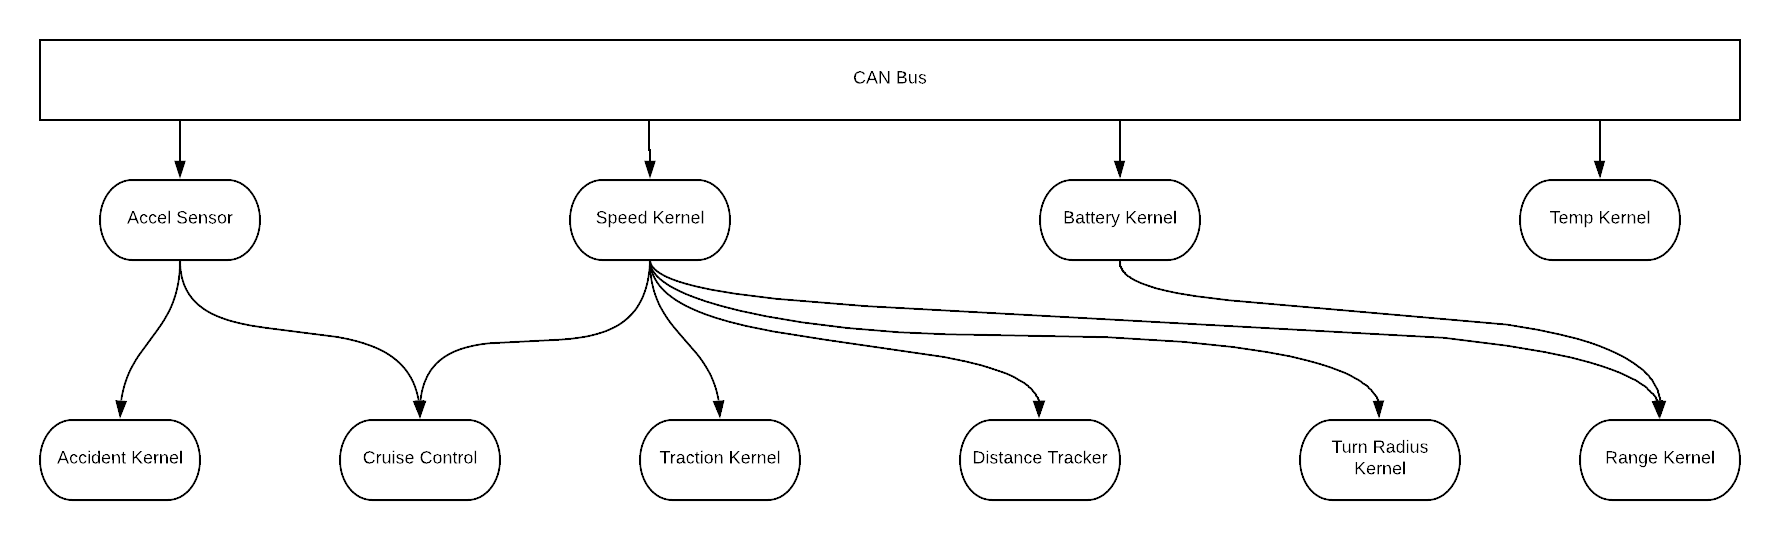
\includegraphics[width=\textwidth]{res/Dependencie_Graph.png}
\end{frame}
\subsection{Dataflowgraph}
\begin{frame}
    \frametitle{Dataflowgraph}
    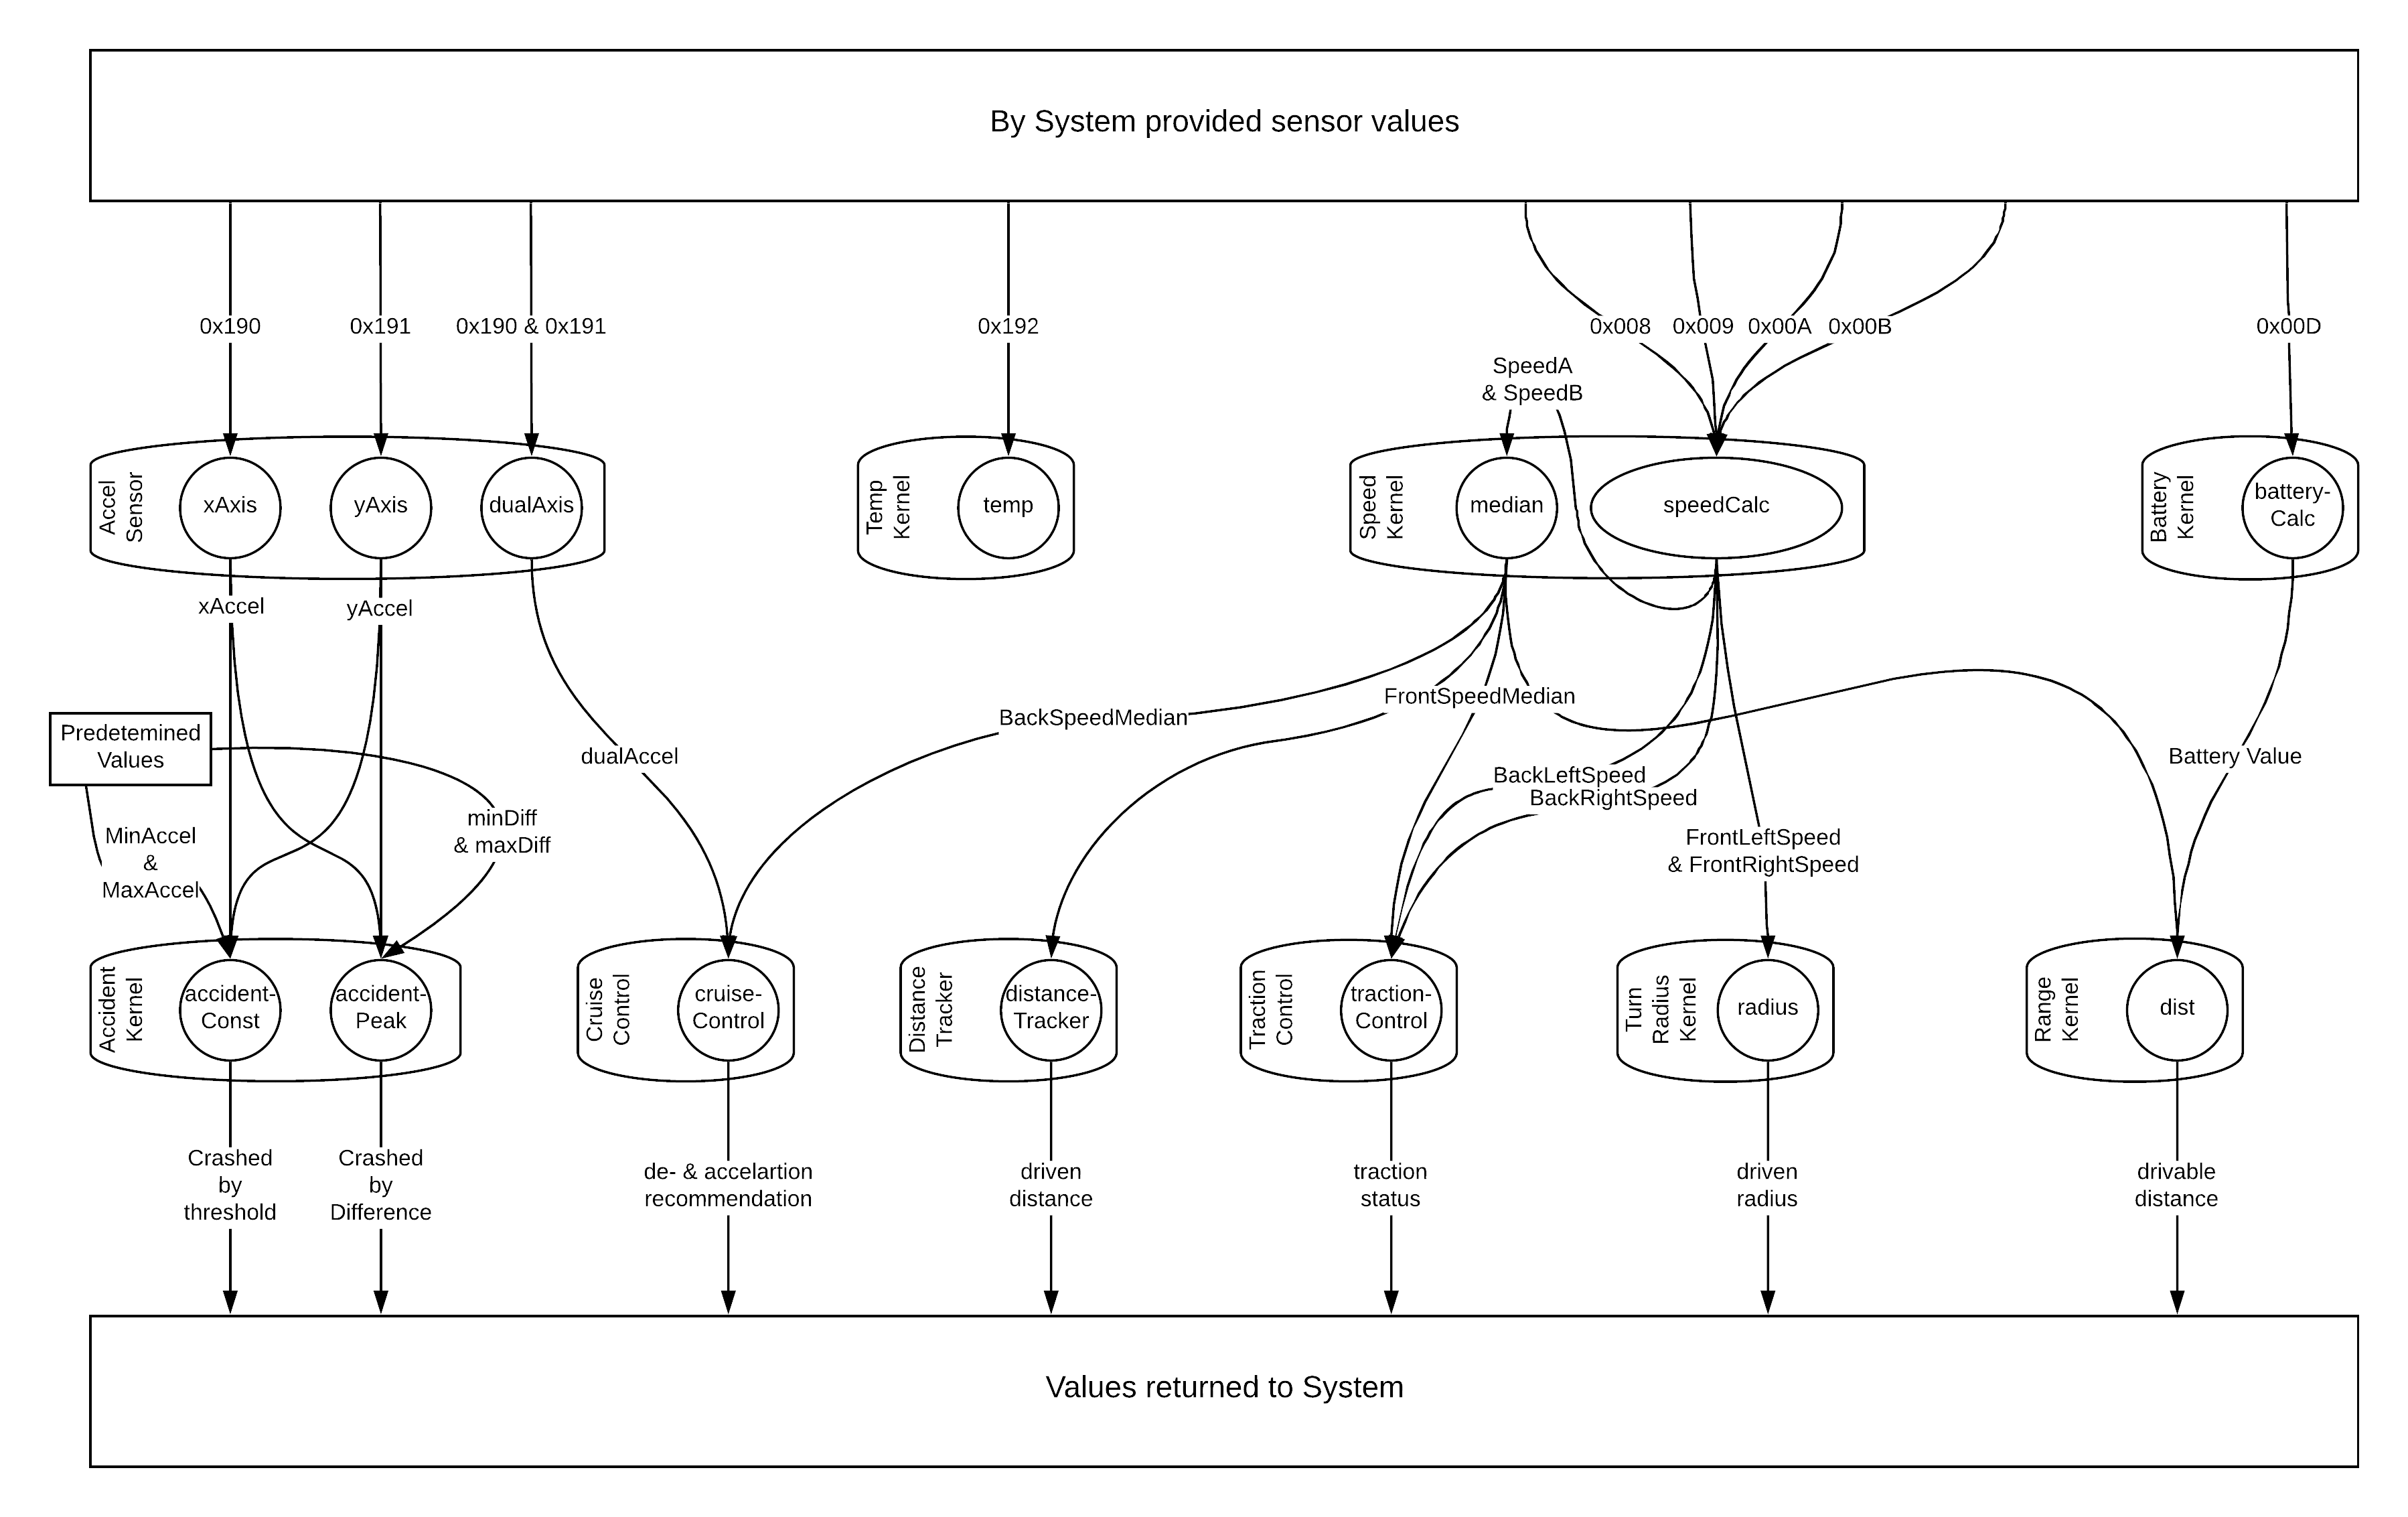
\includegraphics[width=.9\textwidth]{res/Data_Flow_Kernel.png}
\end{frame}
\subsection{Programarchitecture}
\begin{frame}
    \frametitle{Program Flowchart - Big Picture}
    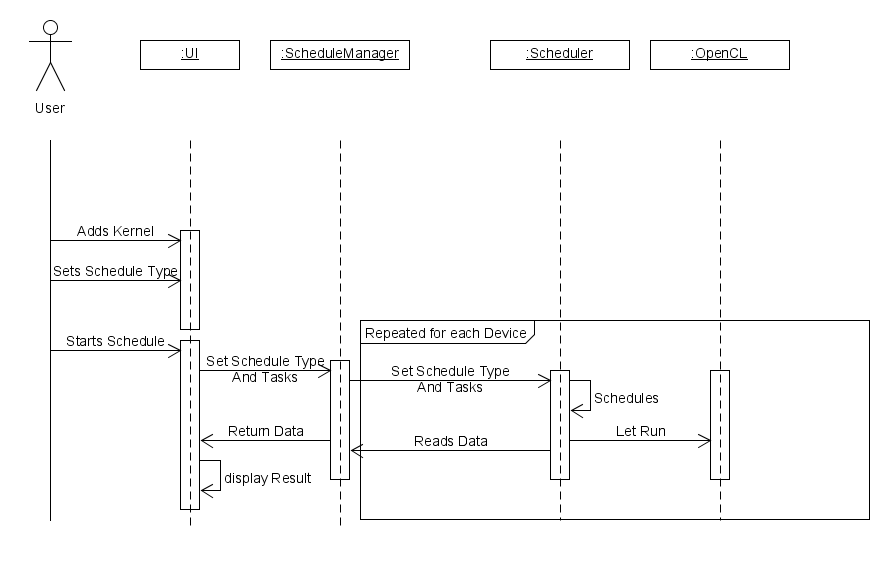
\includegraphics[width=.9\textwidth]{res/Program_Flowchart.png}
\end{frame}
\subsection{UML}
\begin{frame}
    \frametitle{UML - Scheduler}
    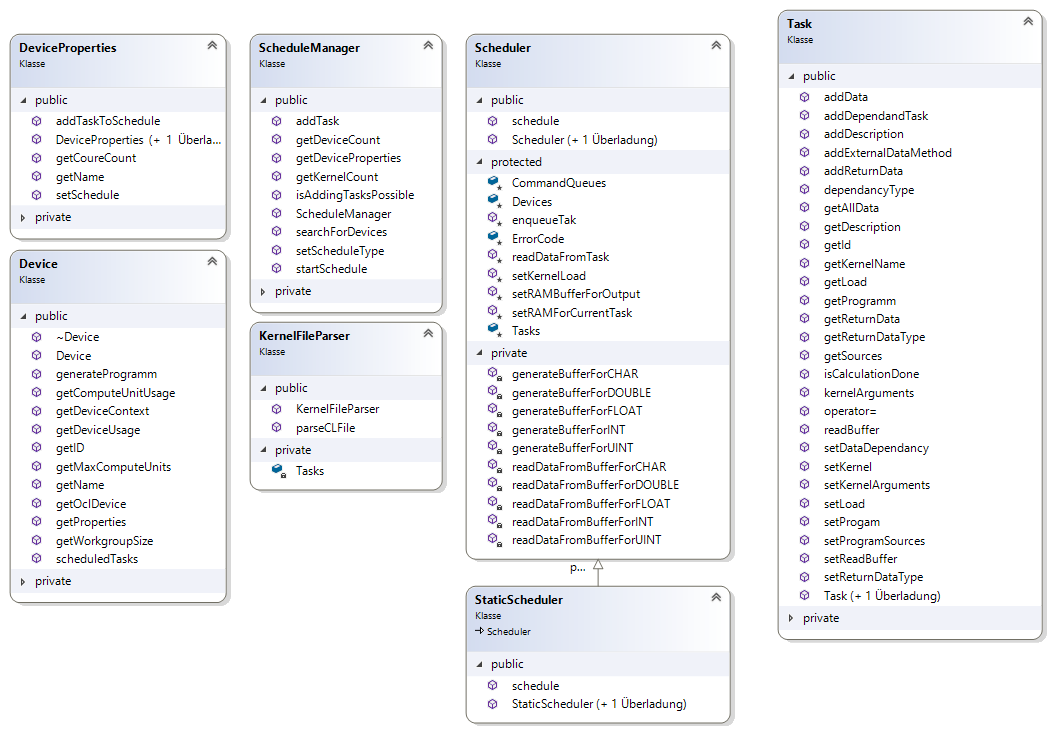
\includegraphics[width=.8\textwidth]{res/ClassDiagramScheduler.png}
\end{frame}
\end{document}
